%%%%%%%%%%%%%%%%%%%%%%%%%%%%%%%%%%%%%%%%%
% This template originates from:
% http://www.LaTeXTemplates.com
%%%%%%%%%%%%%%%%%%%%%%%%%%%%%%%%%%%%%%%%%

%----------------------------------------------------------------------------------------
%	PACKAGES AND OTHER DOCUMENT CONFIGURATIONS
%----------------------------------------------------------------------------------------

\documentclass[11pt]{scrartcl} % Font size

%%%%%%%%%%%%%%%%%%%%%%%%%%%%%%%%%%%%%%%%%
% This template originates from:
% http://www.LaTeXTemplates.com
%%%%%%%%%%%%%%%%%%%%%%%%%%%%%%%%%%%%%%%%%

%----------------------------------------------------------------------------------------
%	PACKAGES AND OTHER DOCUMENT CONFIGURATIONS
%----------------------------------------------------------------------------------------
\usepackage{xcolor}
\usepackage{amsmath, amsfonts, amsthm} % Math packages
\usepackage{minted}
\usepackage{listings} % Code listings, with syntax highlighting
% Umbenennung von Listing auf Auflistung
\renewcommand\listoflistingscaption{Auflistungen}
\usepackage{caption}
\DeclareCaptionLabelFormat{Auflistung}{#1 #2}
\captionsetup[listing]{labelformat=Auflistung, name=Auflistung}


\usepackage{pdflscape}
\usepackage{float} % Enables [H] positioning option for figures

\usepackage[ngerman]{babel} % English language hyphenation
\usepackage{tabularx}
\usepackage{graphicx} % Required for inserting images
\usepackage{hyperref} % for hyperlinks
\providecommand*{\listingautorefname}{Auflistung}
\graphicspath{{Figures/}{./}} % Specifies where to look for included images (trailing slash required)

\usepackage{booktabs} % Required for better horizontal rules in tables

\numberwithin{equation}{section} % Number equations within sections (i.e. 1.1, 1.2, 2.1, 2.2 instead of 1, 2, 3, 4)
\numberwithin{figure}{section} % Number figures within sections (i.e. 1.1, 1.2, 2.1, 2.2 instead of 1, 2, 3, 4)
\numberwithin{table}{section} % Number tables within sections (i.e. 1.1, 1.2, 2.1, 2.2 instead of 1, 2, 3, 4)
\numberwithin{listing}{section} % Number tables within sections (i.e. 1.1, 1.2, 2.1, 2.2 instead of 1, 2, 3, 4)

\setlength\parindent{0pt} % Removes all indentation from paragraphs

\usepackage{enumitem} % Required for list customisation
\setlist{noitemsep} % No spacing between list items

\usepackage{color}

\definecolor{pblue}{rgb}{0.13,0.13,1}
\definecolor{pgreen}{rgb}{0.0,0.5,0}
\definecolor{pred}{rgb}{0.9,0,0}
\definecolor{pgrey}{rgb}{0.46,0.45,48}

%----------------------------------------------------------------------------------------
%	DOCUMENT MARGINS
%----------------------------------------------------------------------------------------

\usepackage{geometry} % Required for adjusting page dimensions and margins

\geometry{
	paper=a4paper, % Paper size, change to letterpaper for US letter size
	top=2.5cm, % Top margin
	bottom=3cm, % Bottom margin
	left=3cm, % Left margin
	right=3cm, % Right margin
	headheight=0.75cm, % Header height
	footskip=1.5cm, % Space from the bottom margin to the baseline of the footer
	headsep=0.75cm, % Space from the top margin to the baseline of the header
	%showframe, % Uncomment to show how the type block is set on the page
}

%----------------------------------------------------------------------------------------
%	FONTS
%----------------------------------------------------------------------------------------

\usepackage[utf8]{inputenc} % Required for inputting international characters
\usepackage[T1]{fontenc} % Use 8-bit encoding

\usepackage{fourier} % Use the Adobe Utopia font for the document

%----------------------------------------------------------------------------------------
%	SECTION TITLES
%----------------------------------------------------------------------------------------

\usepackage{sectsty} % Allows customising section commands

\sectionfont{\vspace{6pt}\normalfont\scshape} % \section{} styling
\subsectionfont{\normalfont\bfseries} % \subsection{} styling
\subsubsectionfont{\normalfont\itshape} % \subsubsection{} styling
\paragraphfont{\normalfont\scshape} % \paragraph{} styling

\usepackage[titles]{tocloft} %customizable table of content

%----------------------------------------------------------------------------------------
%	Hyper Links Setup - Definition of the different links styles
%----------------------------------------------------------------------------------------
\hypersetup{
    colorlinks=true,
    linkcolor=black,
    filecolor=magenta,      
    urlcolor=cyan,
    citecolor=blue,
}

%----------------------------------------------------------------------------------------
%	HEADERS AND FOOTERS
%----------------------------------------------------------------------------------------
\usepackage{fancyhdr}% Required for customising headers and footers
\usepackage[lastpage, user]{zref}
\fancyhf{}
\lhead{HSLU Datenbanksysteme} % Left header
\rhead{Team 4} % right header
%\lfoot{\today} % left footer %% Comment Oli: M.M nach nicht relevant auf jeder Seite
%\rfoot{\thepage/\zpageref{LastPage}} % right footer
\renewcommand{\headrulewidth}{0.5pt}
\renewcommand{\footrulewidth}{0.5pt}
%\usepackage{scrlayer-scrpage} % Required for customising headers and footers

%\ohead*{} % Right header
%\ihead*{} % Left header
%\chead*{} % Centre header

%\ofoot*{} % Right footer
%\ifoot*{} % Left footer
%\cfoot*{\pagemark} % Centre footer

%----------------------------------------------------------------------------------------
%	JAVA CODE STYLE
%----------------------------------------------------------------------------------------

\lstdefinestyle{javaCodeStyle}{
	language=Java, % Use Java functions/syntax highlighting
	frame=single, % Frame around the code listing
	showspaces=false,
	showtabs=false,
	breakatwhitespace=true,
	breaklines=true,
	postbreak=\mbox{\textcolor{red}{$\hookrightarrow$}\space},
	commentstyle=\color{pgreen},
	keywordstyle=\color{pblue},
	stringstyle=\color{pred},	
	basicstyle=\scriptsize,
	showstringspaces=false, % Don't put marks in string spaces
	numbers=left, % Line numbers on left
	numberstyle=\tiny, % Line numbers styling
}

\lstset{style=javaCodeStyle}


\usepackage{minted}
%----------------------------------------------------------------------------------------
%	New Commands
%----------------------------------------------------------------------------------------
%Define texttt with hyphenation enabled
\DeclareTextFontCommand{\mytexttt}{\ttfamily\hyphenchar\font=45\relax}

%For code in text
\newcommand{\code}[1]{\mytexttt{#1}}

%Prevent dots in TOC
\renewcommand{\cftdot}{}

%SubItem for Itemize
\newcommand{\subItem}[1]{
    {\setlength\itemindent{15pt} \item[-] #1}
}


\usepackage[style=numeric,sorting=none]{biblatex}
\usepackage{csquotes}

\usepackage{tcolorbox}
 % Include the file specifying the document structure and custom commands


%----------------------------------------------------------------------------------------
%	TITLE SECTION
%----------------------------------------------------------------------------------------
\title{	
	\begin{figure}[h]
		\begin{flushright}
			
\includegraphics[width=0.2\textwidth]{bilder/hsluLogo.eps}			
		\end{flushright}
	\end{figure}
	\vspace{40pt} % Whitespace
	\normalfont\normalsize
	\textsc{Hochschule Luzern - Informatik}
	\vspace{25pt} % Whitespace
	\rule{\linewidth}{0.5pt}\\ % Thin top horizontal rule
	{\huge Software Testing (SWT)}\\ % The assignment title
	\vspace{10pt} % Whitespace	
	{\large Zusammenfassung von Oliver Amstutz, \today }
	\vspace{12pt} % Whitespace
	\rule{\linewidth}{0.5pt}\\ % Thin top horizontal rule
	\vspace{12pt} % Whitespace
}

\addbibresource{bibtex/refs.bib}

%für pagebreak in Anhang
\newenvironment{longlisting}{\captionsetup{type=listing}}{}

\begin{document}

\pagenumbering{roman}
\rfoot{\thepage} % right footer

%To remove dots in Auflistungen
\makeatletter
\renewcommand\@dotsep{10000}
\makeatother

\maketitle % Print the title
\pagestyle{fancy}
\thispagestyle{empty}
\newpage
\setcounter{page}{1}


\newpage
\tableofcontents
%\newpage
%\listoffigures
%\listoftables
% \renewcommand{\cftdotsep}{\cftnodots}
%\listoflistings

\newpage
\rfoot{\thepage/\zpageref{LastPage}} % right footer
\pagenumbering{arabic}
\section{SW01}

\subsection{Getestet wird immer}
\label{subsec: Getestet wird immer}
Getestet wird immer, es bleibt nur offen:
\begin{itemize}
    \item Wann wird getestet?
    \item Wer testet?
    \item Wo werden die Test Resultate veröffentlicht?
\end{itemize}
Es lohnt sich das Testen vor der Entwicklung einzuplanen (Kosten, Zeitpunkt, Image Schaden).
Beispiele sind:
\begin{itemize}
    \item Unzureichender Last-Test für Ski-Gebiete Online Buchung
    \item Sirenentest musste wegen Systemfehler wiederholt werden 
    \item Oberflächenbehandlungsmaschine welche bereits mit ungenügenden Test geplant wurde (Funktion Düsen nicht interdisziplinär getestet, Positionsensor nicht auf voller Leistung getestet wegen Lärm)
\end{itemize}

\subsection{Die 10er Regel}

Die Abbildung \ref{fig:10er Regel} besagt, dass je weiter ein Fehler sich unentdeckt in die späteren Phasen des Werdeganges eines Produktes oder Prozesses bewegt, umso höher werden die Kosten zur Behebung dieses Fehlers~\cite{sixsigmablackbelt.de}.

\begin{figure}[H]
	\centering
	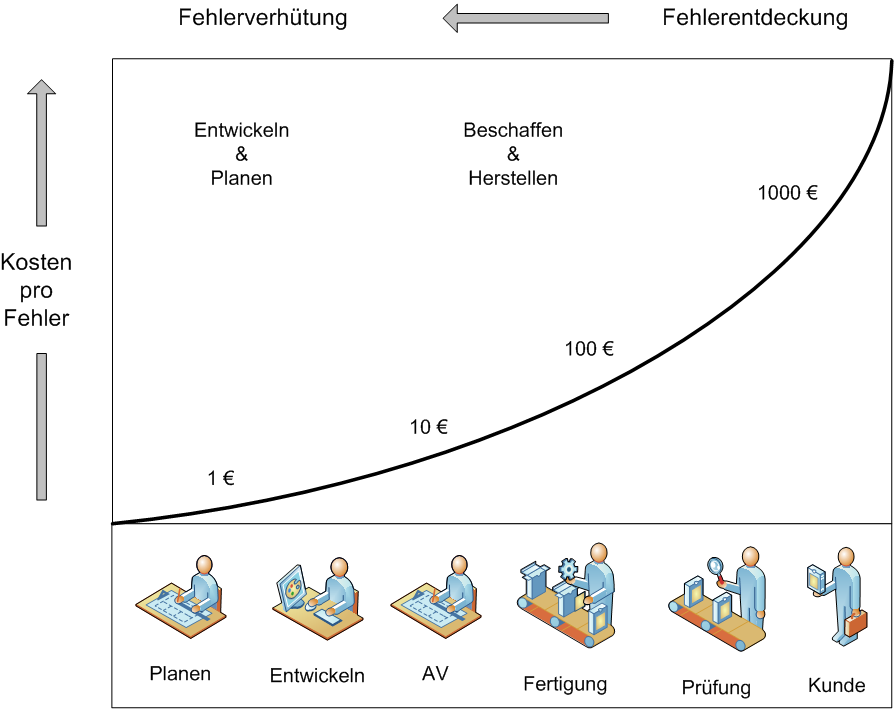
\includegraphics[width=1.0\columnwidth]{01/bilder/Fehlerkosten-10-er-Regel.png}
	\caption{Fehler-kosten der 10er Regel (rule of ten).}
	\label{fig:10er Regel}
\end{figure}

Beispiele:
\begin{itemize}
    \item Beispiele aus Unterkapitel \ref{subsec: Getestet wird immer}
    \item Heroes of Newearth Game-Entwicklung: nicht-Initialisierung einer Variable hat im 64Bit System zum Fehler geführt, welches erst beim Release durch die User bemerkt wurde. Rollback war notwendig.
\end{itemize}

Je früher ein Fehler erkannt wird, desto billiger ist die Behebung!

\subsection{Testen bringt Nutzen}
Mehr Qualität:
\begin{itemize}
    \item wird messbar und quantifizierbar und dadurch sichtbar und verkaufbar
    \item was messbar ist, wird steuerbar
    \item kann somit gezielt gesteigert werden
\end{itemize}

Mehr Wirtschaftlichkeit:
\begin{itemize}
    \item Frühes Erkennen von Fehler ist billiger
    \item After Sales Support wird weniger (Einsparen von Kosten)
    \item Testen dokumentiert Wissen und schützt so Investitionen
    \item Ressourcen werden sinnvoll eingesetzt
\end{itemize}

Risikomanagement:
\begin{itemize}
    \item Risiken werden frühzeitig identifiziert
    \item Risiken werden aktiv gemanagt
    \item Das Eintreffen der Risiken kann vermieden werden
    \item Es wird dort getestet, wo es sinnvoll ist (in der Regel wird das getestet was man: kennt, schon immer getestet hat, gut bekannt ist)
\end{itemize}

Besserer Wettbewerbsvorteil:
\begin{itemize}
    \item keine negativ Presse
    \item hohe Reputation dank Zuverlässigkeit
    \item Erweiterbarkeit und Wartbarkeit ergeben Nachhaltigkeit
    \item swissness, Qualitätsbewusstsein
\end{itemize}


\subsection{Testqualität vs. Produktqualität}
Abbildung \ref{fig: Testqualität vs. Produktqualität} zeigt auf der X-Achse die Testqualität und auf der Y-Achse die Produktqualität~\cite{theNoserWayOfTesting}.

\begin{figure}[H]
	\centering
	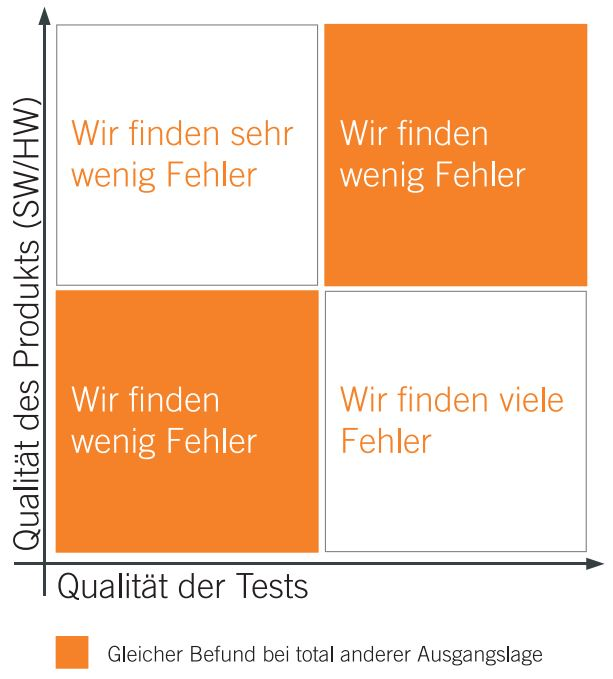
\includegraphics[width=0.6\columnwidth]{01/bilder/Testqualität vs Produktqualität.JPG}
	\caption{Testqualität gegenüber Produktqualität.}
	\label{fig: Testqualität vs. Produktqualität}
\end{figure}

Aus der Abbildung lassen sich folgende Rückschlüsse ziehen:
\begin{itemize}
    \item Testqualität ist entscheidend, nur "halbes Testing" bringt nichts!
    \item Der Grund fürs Testen ist es herauszufinden ob man eine gute oder schlechte Produktqualität hat.
    \item Ist die Testqualität schlecht, können keine Rückschlüsse auf die Produktqualität gewonnen werden -> Provokativ: Warum testet man dann überhaupt?
    \item Man findet sehr wenig Fehler -> gute Entwickler, schlechte Tester
    \item Man findet sehr viele Fehler -> schlechte Entwickler, gute Tester
    \item Aufpassen da man den gleichen Befund haben kann bei total unterschiedlicher Ausgangslage!
    \item Je besser das Testen, desto schlechter erscheint die Produktqualität
    \item Als Konsequenz kann man also sagen - nur die besten testen!
\end{itemize}

Das Bewerten der Fehlerzahl kann über das Messen der gefundenen Fehler im Verlaufe des Projektes bewertet werden. Abbildung \ref{fig: Fehlerkumulation über die Zeit} zeigt das Aufkumulieren der Fehler über die Zeit. Die X-Achse ist die Zeit, die Y-Achse sind alle gefundenen Fehler.

\begin{figure}[H]
	\centering
	\includegraphics[width=0.4\columnwidth]{01/bilder/Fehlerkumulation über die Zeit.JPG}
	\caption{Fehlerkumulation eines SW-Produktes über die Zeit.}
	\label{fig: Fehlerkumulation über die Zeit}
\end{figure}

Wenn der Gradient der gefundenen Fehler (rote Linien) flacher wird, ist dies ein Zeichen dafür, das mit den angewandten Methoden keine weiteren Fehler gefunden werden können. Das kann auch so interpretiert werden, das in Abbildung \ref{fig: Testqualität vs. Produktqualität} man die Qualität des Produktes gesteigert hat. Das sich die Qualität der Tests verschlechter über Zeit wird nicht angenommen.
Weitere Info's zu diesem Thema in Kapitel \textcolor{red}{Noch zu definieren - später!}.

\subsection{Anforderungen der Stakeholder}
Stellen Sie sich ein Glas / Ball vor. Ich kann ein Glas/Ball nicht testen ohne die Anforderungen der Stakeholder zu kennen. Dies beinhaltet:
\begin{itemize}
    \item Anwendungszweck
    \item Umgebung
    \item Bedürfnisse
    \item Kontext
\end{itemize}

Ein Softwaretest prüft und bewertet Software auf Erfüllung der für ihren Einsatz definierten Anforderungen und misst ihre Qualität. Fürs Testen braucht's Erwartungen, Anforderungen und Akzeptanzkriterien!

\textcolor{red}{Noch am passenden Ort einfüllen:}
Code qualität bei der Entwicklung bereits prüfen mit:
\begin{itemize}
    \item 4 Augen Prinzip
    \item Codereview
    \item Pair-Programming
\end{itemize}

Die erste Teststufe liegt bereits beim Software Entwickler!

\section{SW02}


\subsection{Testen vs Experimentieren}

Testen unterscheidet sich von Experimentieren dadurch, dass es beim Testen eine Erwartung gibt die belegt werden soll, während das Ergebnis beim Experimentieren offen ist oder nur vermutet werden kann:
\begin{itemize}
    \item Anforderungen (= erwartetes Verhalten) müssen bekannt sein
    \item Testen bedingt Anforderungen und prüft auf Unterschiede
    \item ohne Anforderungen ist Testen schwierig bis unmöglich
    \item Der Kontext vom Testen ist wichtig (Formale Nachweise, zb für Flugzeugindustrie, benötigen einen viel höheren formellen Aufwand für das selbe in einem anderen Kontext)
\end{itemize}

\subsection{Agiles Testen}

Vorteile von agilem Vorgehen:
\begin{itemize}
    \item kurze Zyklen bringen schnell Feedback
    \item CI / CD unterstützen schnelles Feedback
    \item Jede Teillieferung bringt Nutzen
    \item Wichtiges erfolgt zuerst
\end{itemize}

Gefahren bei agilem Vorgehen:
\begin{itemize}
    \item Ganzheitlicher (Test-) Ansatz fehlt (= keine Teststrategie)
    \item Keine Negativ-Tests
    \item Keine Grenzwerttests
    \item Keine NFA – Tests (Nicht Funktionale Anforderungen)
    \item Automatisierung erfolgt zu spät weil Produkt zulange instabil ist
\end{itemize}

Aus Test Sicht wichtige Punkte welche Aufmerksamkeit benötigen beim agilen Vorgehen:
\begin{itemize}
    \item PO hat (zu) grosse Verantwortung (und oft wenig bis kein Testwissen)
    \item Ein Team kann «Alles», jede und jeder im Team können «Alles»
    \item Es gibt Akzeptanzkriterien (AK)
    \item Es gibt eine DOD (Definition of Done) und teilweise eine DOR (Definition of Ready: Wenn die Product Backlog Items "ready" für den Sprint sind~\cite{scrum-events.de})
    \item Es darf / muss Teststories\footnote{Teststory ist ein Bestandteil einer User Story. Weiter Bestandteile können sein: Technical Story, Infrastructure Story, ...} geben, diese beinhalten folgende Tätigkeiten:
    \begin{itemize}
        \item Codereview
        \item Testanalyse (Was muss getestet werden)
        \item Testdesign (Wie wird getestet, wie sieht der Testablauf aus)
        \item Tests bauen (auch automatisierte)
        \item Testdaten (Passende, realistische Testdaten definieren und bereitstellen)
        \item Tests durchführen
    \end{itemize}   
\end{itemize}

\subsection{Rollen/Tätigkeiten im Testing}

Abbildung \ref{fig:Rollen im Testing} zeigt einen Vorschlag von möglichen Rollen mit den jeweiligen Verantwortlichkeiten und notwendigen Skill Set.

\begin{figure}
\centering
\begin{minipage}{.47\textwidth}
  \centering
  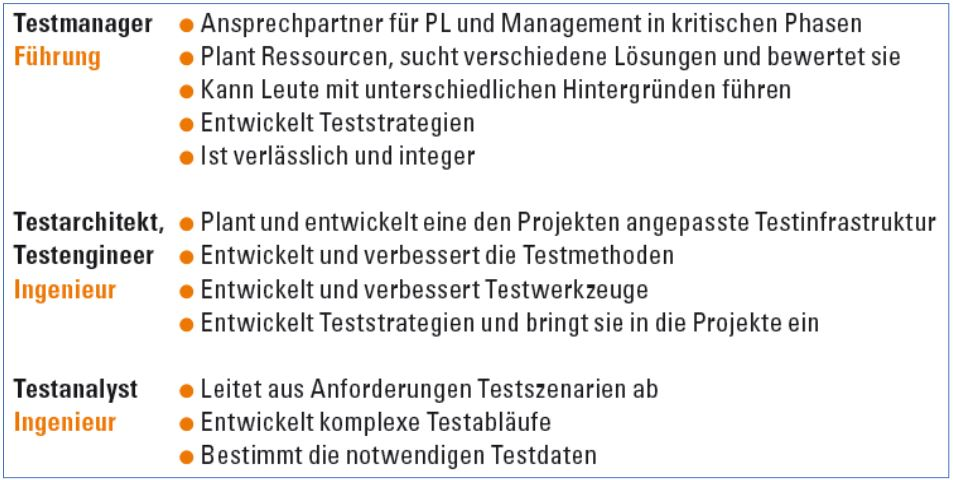
\includegraphics[width=1\linewidth]{02/bilder/Taetigkeiten Testing 1.JPG}
\end{minipage}%
\begin{minipage}{.53\textwidth}
  \centering
  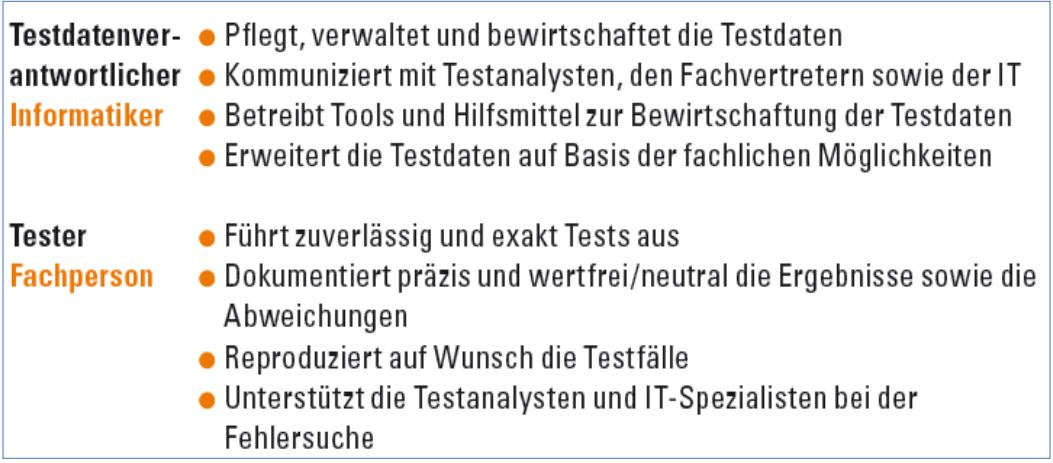
\includegraphics[width=1\linewidth]{02/bilder/Taetigkeiten Testing 2.JPG}
\end{minipage}
	\caption{Vorschlag von 5 möglichen Rollen/Tätigkeiten im Testing.}
	\label{fig:Rollen im Testing}
\end{figure}

\subsection{Test-Prozess}

Prozesse definieren Abläufe, Rollen und Verantwortlichkeiten klären. Orientiert man sich beim Testen an einem Prozess, wird sichergestellt, dass Tests:
\begin{itemize}
    \item geplant
    \item vorhersehbar
    \item gesteuert
    \item nachvollziehbar
    \item systematisch
\end{itemize}
sind. Es soll dabei beachtet werden das der Prozess nur ein Hilfsmittel ist. Beispiel: Zertifizierte Schwimmwesten aus Beton sind zwar nach Prozess erzeugt, jedoch überhaupt nicht zweckmässig. Abbildung \ref{fig:Einordnung Testprozess} zeigt eine Übersicht, wo der Testprozess einzuordnen ist.

\begin{figure}[H]
	\centering
	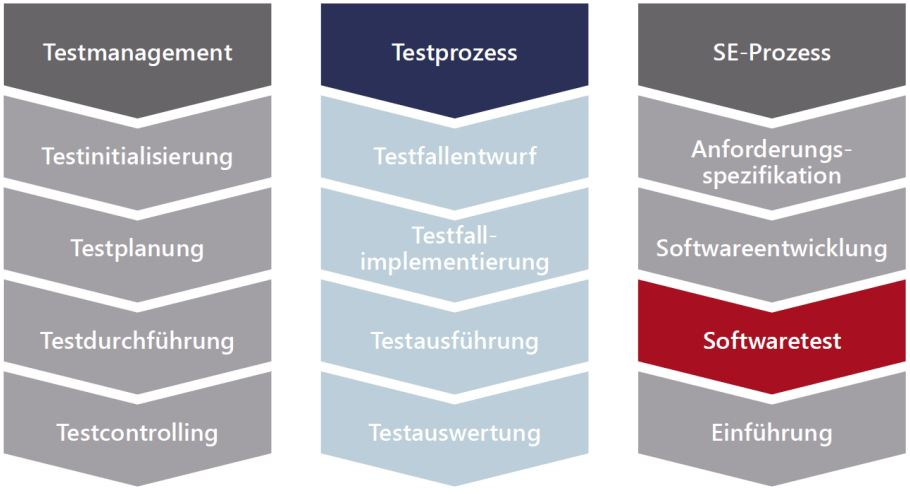
\includegraphics[width=0.7\columnwidth]{02/bilder/Einordnung Testprozess.JPG}
	\caption{Übersicht, wo der Testprozess in der Software Entwicklung (SE) Einzuordnen ist.}
	\label{fig:Einordnung Testprozess}
\end{figure}

Nachfolgend in Abbildung \ref{fig:Phasen des Testings} sind die vier Phasen des Testen's gezeigt.

\begin{figure}
    \centering
    \begin{minipage}{.48\textwidth}
        \centering
        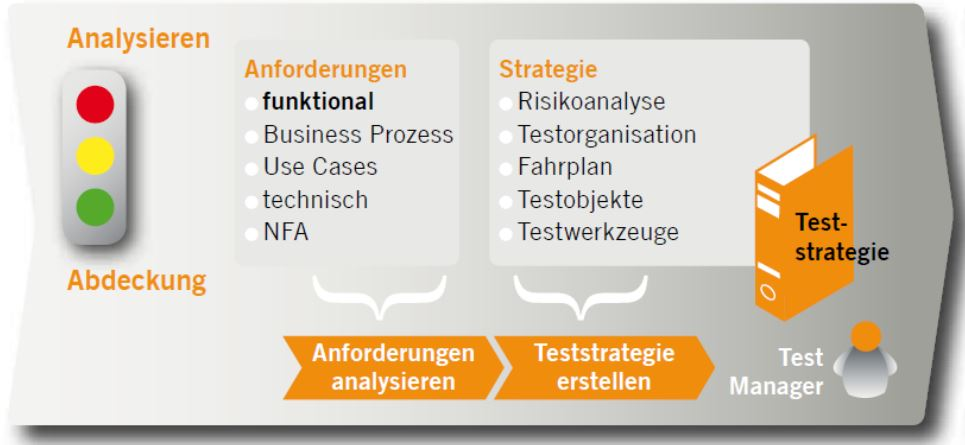
\includegraphics[width=1\linewidth]{02/bilder/Testprozess1.JPG}
        \caption{Phase 1: Analysieren.} 
        \vspace{2ex}
    \end{minipage}
    \begin{minipage}{.48\textwidth}
        \centering
        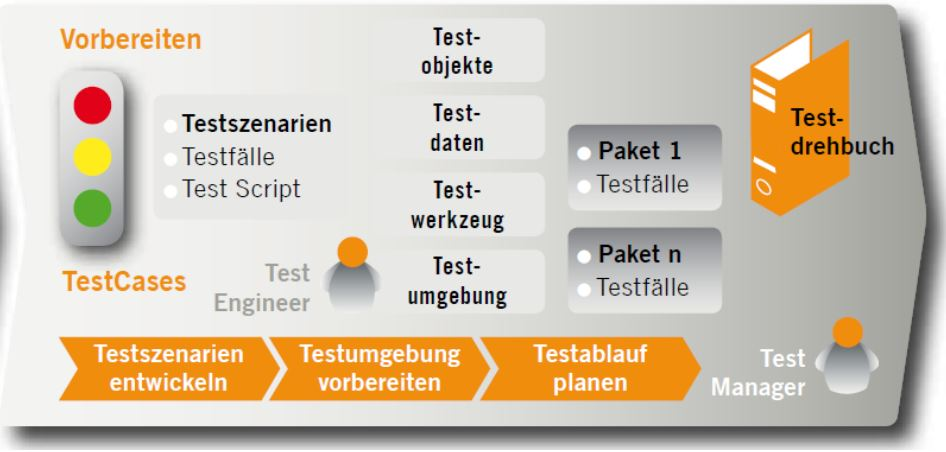
\includegraphics[width=1\linewidth]{02/bilder/Testprozess2.JPG}
        \caption{Phase 2: Vorbereiten.} 
        \vspace{2ex}
    \end{minipage}
    \begin{minipage}{.48\textwidth}
        \centering
        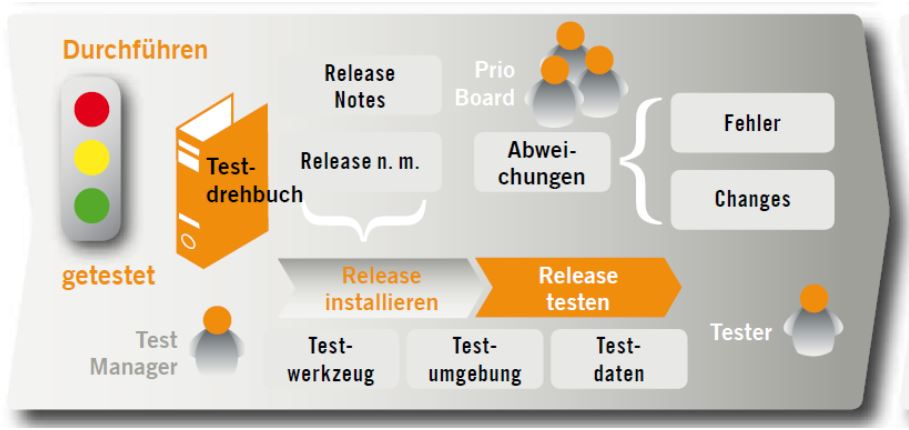
\includegraphics[width=1\linewidth]{02/bilder/Testprozess3.JPG}
        \caption{Phase 3: Durchführen.} 
        %\vspace{4ex}
    \end{minipage}
    \begin{minipage}{.48\textwidth}
        \centering
        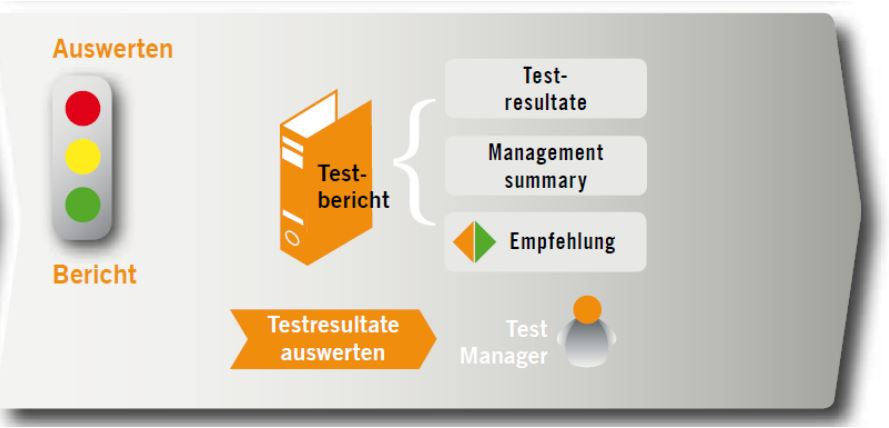
\includegraphics[width=1\linewidth]{02/bilder/Testprozess4.JPG}
        \caption{Phase 4: Auswerten.} 
        %\vspace{4ex}
    \end{minipage}
	\caption{Die 4 Phasen des Testprozesses von Noser~\cite{theNoserWayOfTesting}.}
	\label{fig:Phasen des Testings}
\end{figure}

\subsection{Testprozess, Phase 1: Analysieren}

Abbildung \ref{fig:Testprozess Phase 1} zeigt die Details in Phase 1.

\begin{figure}[H]
	\centering
	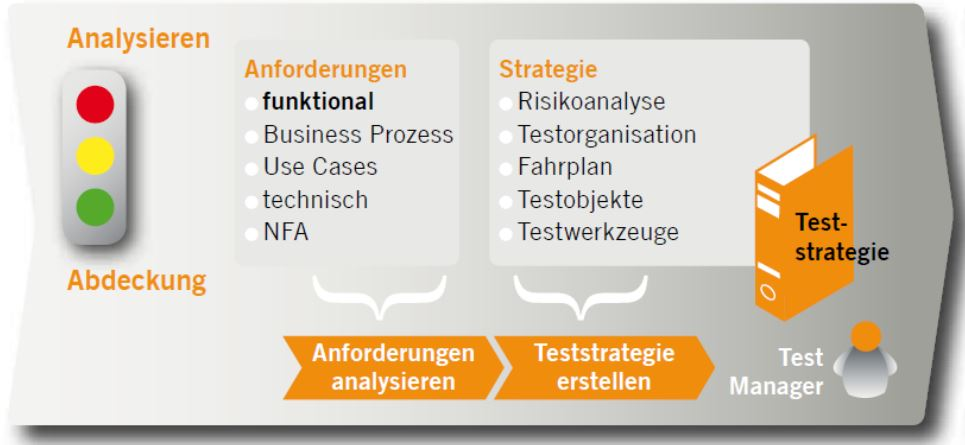
\includegraphics[width=0.8\columnwidth]{02/bilder/Testprozess1.JPG}
	\caption{Phase 1: Abdeckung Analysieren.}
	\label{fig:Testprozess Phase 1}
\end{figure}

\subsection{Teststrategie}
Grundsätzlich bestimmt eine Teststrategie, ob, was und wie tief getestet werden soll. Die Teststrategie bestimmt das Test-Ziel und weist dessen Nutzen aus. Mit der Teststrategie setzt man Prioritäten, welche Bereiche wichtig sind zu testen. Prioritäten setzt man, da man weder unendlich Zeit noch unendlich Geld hat.

Aus folgenden Fragen kristallisiert sich die Teststrategie:
\begin{itemize}
    \item Was kann im Fehlerfall passieren? (Menschenleben, Gesundheit, Umwelt, Reputation)
    \item Frage der Haftung und Garantie? (Nach EU Recht hat man 2 Jahre Garantie auf SW!)
    \item Wie lange «lebt» das Projekt / Produkt?
    \item In welchem Umfeld wird es eingesetzt? (Bsp: Billetautomaten Regen + Touch Screen / Sonneneinfall + Sichtbarkeit von Screen)
    \item Wie «komplex» ist das Produkt?
    \item Was kostet das Produkt? (Testen muss im Verhältnis sein zum erwarteten Umsatz)
    \item Gibt es Gesetze , Vorschriften oder Normen? (Datenschutz) (Kann man typischerweise nur mit Tests belegen)
    \item Welchen «Standard» haben vergleichbare Produkte? (tieferer Standart als die Konkurrenz erschwert den Markteinstieg)
    \item In welcher «Liga» wird das Produkt lanciert? (Budget vs Premium)
    \item Wie «sicher» soll oder muss das Produkt sein?
\end{itemize}

\subsection{Übung: Test-Strategie in 15 Minuten}

Abbildung \ref{fig:Teststrategie in 15 min} zeigt eine Hilfestellung um eine Test-Strategie in 15 Minuten zu entwickeln.

\begin{figure}[H]
	\centering
	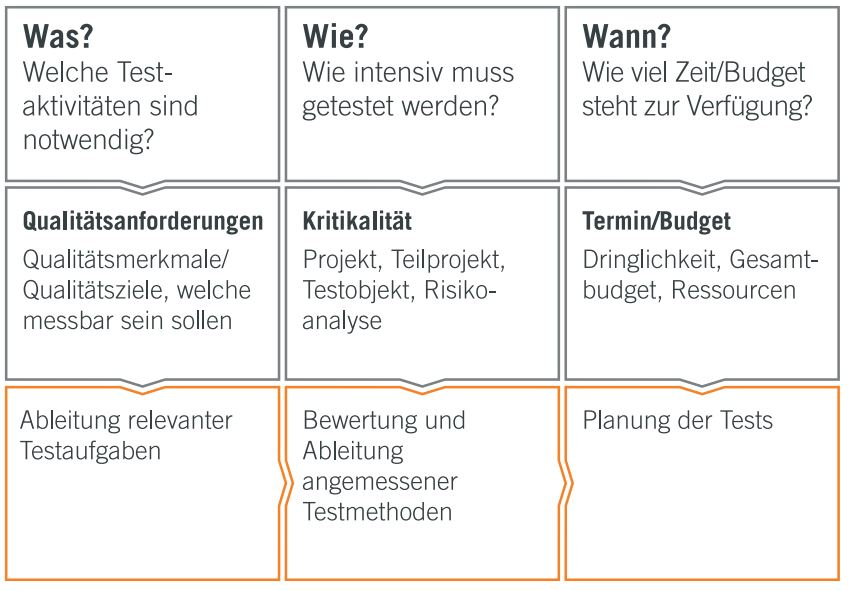
\includegraphics[width=0.6\columnwidth]{02/bilder/Teststrategie in 15 min.JPG}
	\caption{Hilfestellung für eine Test-Strategie in 15 Minuten~\cite{theNoserWayOfTesting}.}
	\label{fig:Teststrategie in 15 min}
\end{figure}

Beispiel Teststrategie für Game:
\begin{itemize}
    \item Welche Testaktivitäten sind notwendig? Das Spiel soll flüssig (NFT) und ohne Game Play beeinträchtigende Fehler spielbar sein. Daraus sind folgende relevanten Testaufgaben abgeleitet:
    \begin{itemize}
        \item Performance Test auf handelsüblichen Geräten
        \item Game Play Tests (Alpha /Beta Tests) um allfällige Fehler zu finden
    \end{itemize}
    \item Wie intensiv muss getestet werden? Das Risiko ist sehr tief, einzig die Gefahr besteht das aufgrund von zu vielen Fehlern die Motivation zum entwickeln reduziert.
    \begin{itemize}
        \item Beim entdecken von Bugs zuerst Tests schreiben welche diese Bugs Beschreiben und Ihn und ähnliche Bugs entdecken
        \item Komplizierte Konzepte und Anordnungen vorgängig (TDD) testen, da man sicher sein kann, viele Bugs im Code zu haben
    \end{itemize}
    \item Wie viel Zeit/Budget steht zur Verfügung? Da dies ein Freizeit Projekt ist, hat man weder Zeit noch Geld. Die einzig verfügbare Ressource ist die Motivation, welche die resultierende Zeit bestimmt. Eine hohe Motivation kommt von einem Funktionierenden Prototypen und neuen Features.
\end{itemize}
%\include{3_Datenmodellierung/datenmodellierung}
%\include{4_Datenbanksprache/datenbanksprache}
%\include{5_Systemarchitektur/systemarchitektur}
%\include{6_Resultate/resultate}
%\include{7_Rückblick/rückblick}
\printbibliography
%\include{9_Appendix/appendix}

%\bibliography{./bibtex/refs}
%\bibliographystyle{plain} %ieeetr}

\end{document}
